\documentclass[12pt]{article}
\usepackage[utf8]{inputenc}
\usepackage{geometry}
\usepackage{svg}
\usepackage{float}
\usepackage{caption}
\usepackage{amsmath,amsthm,amsfonts,amssymb,amscd}
\usepackage{fancyhdr}
\usepackage{titlesec}
\usepackage{hyperref}
\usepackage{listings}
\usepackage[skip=3pt]{parskip}
\usepackage[ngerman]{babel}
\pagestyle{empty}
\titleformat*{\section}{\large\bfseries}
\titleformat*{\subsection}{\bfseries}

%
\geometry{
	a4paper,
	total={170mm,240mm},
	left=20mm,
	top=30mm,
}

\date{}
%Bitte ausfüllen
\newcommand\course{Betriebssysteme}
\newcommand\hwnumber{\large Portfolio 1}
\newcommand\Name{Fabian Sponholz}
\newcommand\Neptun{1561546}

%Matheinheiten
\newcommand\m{\:\textrm{m}}
\newcommand\M{\:\Big[\textrm{m}\Big]}
\newcommand\mm{\:\textrm{mm}}
\newcommand\MM{\:\Big[\textrm{mm}\Big]}
\newcommand\un{\underline}
\newcommand\s{\:\textrm{s}}
\newcommand\bS{\:\Big[\textrm{S}\Big]}
\newcommand\ms{\:\frac{\textrm{m}}{\textrm{s}}}
\newcommand\MS{\:\Big[\frac{\textrm{m}}{\textrm{s}}\Big]}
\newcommand\mss{\:\frac{\textrm{m}}{\textrm{s}^2}}
\newcommand\MSS{\:\Big[\frac{\textrm{m}}{\textrm{s}^2}\Big]}

%Trennlinie
\newcommand\separator{\rule{\linewidth}{0.5pt}}

%Bitte nicht einstellen
\renewcommand{\figurename}{Abbildung}
\renewcommand{\tablename}{Tabelle}
\pagestyle{fancyplain}
\headheight 35pt
\lhead{\Name\\\Neptun}
\chead{\textbf{ \hwnumber}}
\rhead{\course \\ \today}
\lfoot{}
\cfoot{}
\rfoot{\small\thepage}
\headsep 1.5em

\begin{document}
	
\section*{Aufgabe 1 - System Call}
Der Source Code der System-Call-Wrapper befindet sich in der \texttt{glibc} Bibliothek.
Genauer gesagt in der Datei \texttt{sysdeps/unix/sysv/linux/read.c}. Dort wird die generische Funktion \texttt{SYSCALL\_CANCEL} mit der Nummer des entsprechenden Systemcalls aufgerufen:

\begin{lstlisting}[language=c]
/* Read NBYTES into BUF from FD.  Return the number read or -1.  */
ssize_t
__libc_read (int fd, void *buf, size_t nbytes)
{
	return SYSCALL_CANCEL (read, fd, buf, nbytes);
}

\end{lstlisting}

Im Linux-Kernel findet sich die Gegenstelle \texttt{fs/read\_write.c}: 
\begin{lstlisting}[language=c]
SYSCALL_DEFINE3(read, unsigned int, fd, char __user *, buf, size_t, count)
{
	return ksys_read(fd, buf, count);
}
\end{lstlisting}
Dort wird der entsprechende System-Call, der in einer System-Call-Tabelle einer architekturspezifischen System-Call-Nummer zugeordnet ist, ausgeführt.

Der gesamte Verlauf bei Aufruf des System-Calls \emph{read()} ist dann wie folgt:

\begin{enumerate}
	\item User Space:
	\begin{itemize}
		\item Der Wrapper read() in der glibc ruft syscall(SYS\_read, ...) auf.
		\item Dabei wird die System-Call-Nummer SYS\_read und die Argumente (z.B. Dateideskriptor, Puffer, Anzahl der Bytes) übergeben.
	\end{itemize}
	
	
	\item Übergang in den Kernel Space:
	\begin{itemize}
		\item Ein Software-Interrupt wird ausgelöst.
		\item Der CPU-Modus wechselt in den Kernel-Modus.
	\end{itemize}
	
	
	\item Kernelraum (System Call Handler):
	
	\begin{itemize}
		\item Der System-Call-Dispatcher sucht anhand der System-Call-Nummer die entsprechende Implementierung, z.B. SYSCALL\_DEFINE3(read, ...).
		\item Die Implementierung (z.B. ksys\_read()) verarbeitet den Aufruf und ruft weitere Kernel-Subsysteme wie das Virtual File System (VFS) auf.
	\end{itemize}
	
	
	\item Rückkehr in den Benutzerraum:
	
	\begin{itemize}
		\item Nach Abschluss des System-Calls kehrt die Kontrolle zurück in den Benutzerraum, und das Ergebnis wird an die Anwendung zurückgegeben.
	\end{itemize}
	
\end{enumerate}

\section*{Aufgabe 2 - System Call Latenz}
Der Versuchsaufbau ist recht simpel: Es wird einfach die Zeit gemessen, die für die Verarbeitung eines möglichst einfachen System-Calls benötigt wird. Dafür wird die Zeit zu Begin der Verarbeitung genommen und von der Zeit nach der Verarbeitung subtrahiert. Der ganze Prozess wird 1000000 mal wiederholt und aus diesen Iterationen der Minimalwert bestimmt.

Als Kandidat für den System-Call, der gemessen wird, habe ich mich für \texttt{getpid()} entschieden. Seit glibc Version 2.25 wird die PID hier auch nicht mehr im Cache gespeichert, sondern bei jedem Aufruf der entsprechende System-Call ausgeführt. Da \texttt{getpid()} keine aufwendigeren Operationen wie z.B. Dateisystem-Zugriffe benötigt, eignet er sich besonders gut für dieses Experiment.

Aus Interesse habe ich zusätzlich noch die \emph{maximale} Latenz gemessen.

Auf meinem Laptop (Prozessor: Intel i7-6700HQ (4x3,5 GHz), Kernel: Linux 6.12.1, Glibc Version 2.40) betrug die minimale gemessene Latenz \textbf{ca. 850 ns}. Die Maximale Latenz variierte stark und lag bei mehreren Programmausführungen jeweils zwischen 50.000 ns und 700.000 ns.

Die Latenz von System-Calls ist in erster Linie von der Hardware (CPU, RAM) und dem verwendeten Kernel abhängig. Zudem wird sie auch ggf. durch Hintergrundprozesse beeinflusst: daher stammt vermutlich auch die starke Abweichung zwischen Minimal- und Maximalwert. In einer isolierten Umgebung ohne jegliche Hintergrundprozesse sollte es keine solchen Ausreißer geben.

\section*{Aufgabe 3 - Kontextwechsel}
\subsection*{Was ist ein Kontextwechsel?}
Ein Kontextwechsel tritt auf, wenn die CPU von einem Prozess oder Thread zu einem anderen wechselt. Dabei müssen alle Informationen des aktuellen Prozesses (z. B. Register, Program Counter, Speicherzuordnung) gesichert und die des neuen Prozesses geladen werden. Der dabei entstehende Zeitaufwand wird als \emph{direkte Kosten} bezeichnet.

\subsection*{Messung der Latenz von Kontextwechseln}
Um die Latenz von Kontextwechseln zu messen, muss zunächst ein Weg gefunden werden, einen Kontextwechsel zu erzwingen. Hier gibt es bereits eine bewährte Technik, die auch in Benchmark-Tools wie z.B. \emph{lat\_ctx} verwendet wird. Dabei werden Daten zwischen mehreren Prozessen oder Threads mit Hilfe von zyklischen Pipes im Kreis gesendet. So wird bei jedem Lese-/Schreibprozess in die Pipe ein Kontextwechsel erzwungen.

In diesem Fall habe ich zu diesem Zweck ein C-Programm entwickelt, das eine zyklische Pipe zwischen einem Thread und dem Haupt-Thread simuliert. Immer, wenn der Haupt-Thread Daten schreibt, werden diese vom Neben-Thread gelesen und wieder zurückgeschrieben. Dann werden sie vom Haupt-Thread wiederum gelesen und das ganze beginnt von vorne.

Der ganze Prozess wird bei meinem Testprogramm 1000000 mal ausgeführt, wodurch 2000000 Kontextwechsel provoziert werden. Am Ende wird die vergangene Zeit durch 2000000 geteilt und somit die durchschnittliche Dauer eines Kontextwechsels angenähert.

Die hiermit gemessene Latenz liegt bei \textbf{ca. 3000 ns}.

\subsection*{Benchmark- und Profiling-Tools}
Zunächst einmal habe ich die stattfindenden Kontextwechsel in meinem Testprogramm validiert, indem ich das Profiling-Werkzeug \emph{perf} verwendet habe. Ich habe hier folgenden Befehl verwendet:

\texttt{sudo perf stat -e context-switches ./ctx\_latency}

Durch \texttt{perf} werden etwa 1000000 Konzextwechsel festgestellt. Dies zeigt, dass der Mechanismus zum Erzwingen von Kontextwechseln funktioniert. Hier können nicht alle Kontextwechsel erkannt werden, da perf mit einer \emph{Sampling-Rate von etwa 4000 Hz} arbeitet und somit nicht alle Kontextwechsel erkennen kann.

Als bekanntestes Benchmark-Tool zum Bestimmen der Latenz fällt \emph{lmbench} mit dem Benchmark \texttt{lat\_ctx} ins Auge, der ähnlich vorgeht wie meine Implementierung. Hier werden allerdings Subprozesse mit zyklischen Pipes verbunden, anstelle von Threads.

Leider kompiliert lmbench mit meinen aktuellen Bibliotheken nicht, daher konnte ich leider keine Ergebnisse vergleichen.

Ein weiteres Tool, mit dem man Kontextwechsel beobachten kann, ist \texttt{htop}. Hier kann man die Kontextwechsel pro Sekunde beobachten, nicht jedoch die Summe.

\begin{figure}[H]
	\centering
	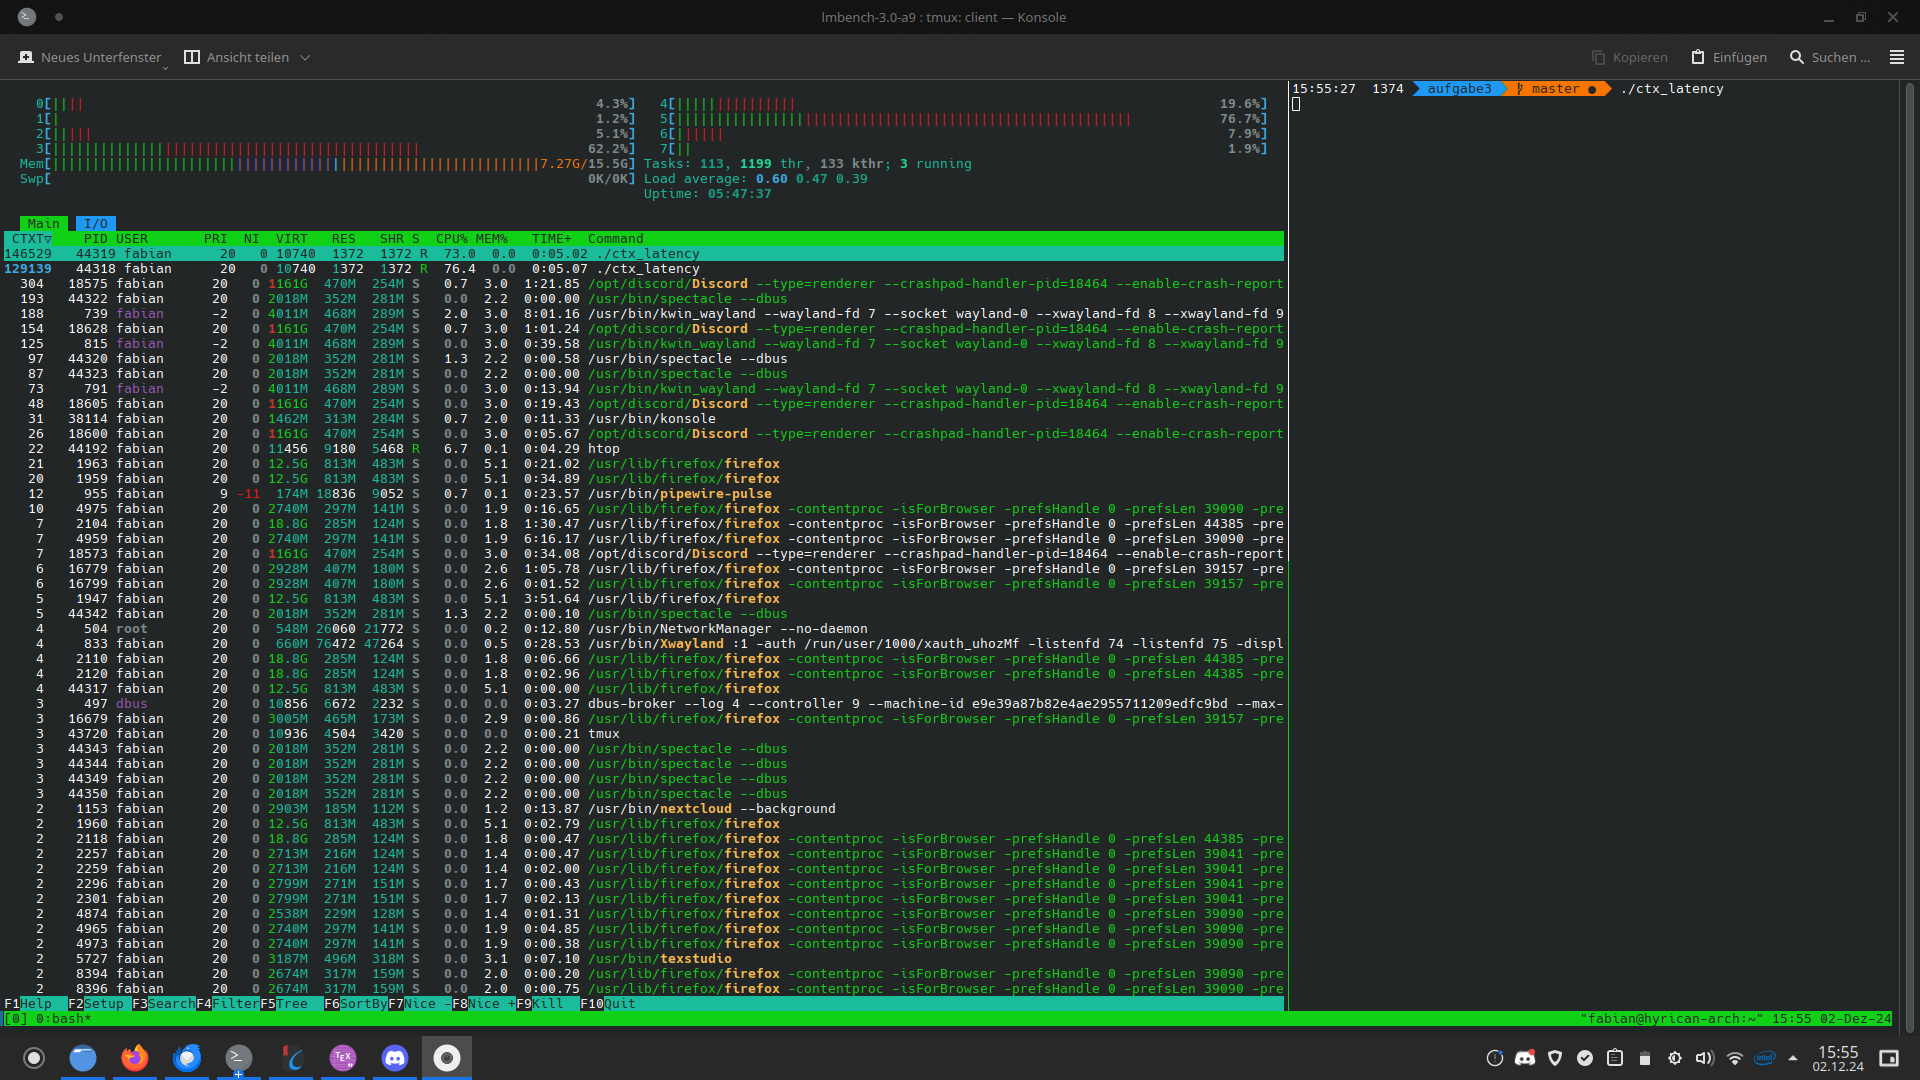
\includegraphics[width=\textwidth]{./img/screenshot_htop_ctx}
	\caption{Beobachten der Kontextwechsel mit htop}
\end{figure}

\subsection*{Indirekte Kosten von Kontextwechseln}
Folgende Faktoren sind maßgeblich für die indirekten Kosten von Kontextwechseln:

\begin{itemize}
	\item Cache Misses:
	Der CPU-Cache muss möglicherweise neu geladen werden, da der neue Prozess andere Daten benötigt.
	
	\item TLB-Flushes:
	Die Translation Lookaside Buffer (TLB), der virtuelle Adressen zwischenspeichert, wird bei einem Adressraumwechsel ungültig gemacht.
	
	\item Pipeline-Stalls:
	Die CPU-Pipeline wird entleert, da neue Instruktionen geladen werden müssen.
\end{itemize}

Anwendungen mit vielen Kontextwechseln können stark durch die indirekten Kosten beeinflusst werden, insbesondere wenn auf großen Datenmengen gearbeitet wird und hier unnötig viele Threads um die entsprechenden CPU-Ressourcen konkurrieren.

Ein möglicher Optimierungsansatz in diesem Fall wäre die Beschränkung von Worker-Threads auf die Anzahl der tatsächlich verfügbaren CPU-Kerne. So werden unnötige Kontextwechsel und die damit einhergehenden Kosten vermieden.
\end{document}